\documentclass[12pt]{article}
\usepackage[utf8]{inputenc}
\usepackage{amsmath}
\usepackage{amssymb}
\usepackage{graphicx}

\graphicspath{ {./plots/} }

\newcommand{\rectres}[1]{
\begin{center}
\begin{tabular}{ |c| }
\hline\\
#1\\
\\
\hline
\end{tabular}
\end{center}
}

\newcommand{\qed}{\hfill$\blacksquare$}

\title{Introduction to Numerical Optimization\\Assignment 3}
\author{Yair Nahum 034462796\\and\\blabla 11111111 }

\begin{document}

\maketitle

%\tableofcontents{}

\section{Quasi-Newton Methods}

\subsection{BFGS Method Implementation}
Implementation in code
\subsection{Find  the  Minimum  of  the  Rosenbrock  Function}
Implementation in code\\
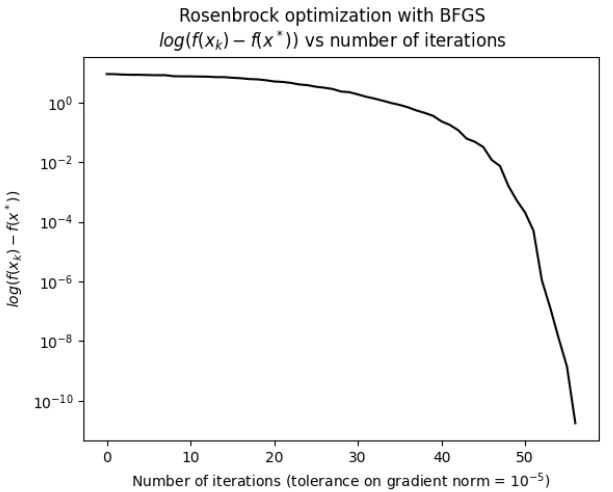
\includegraphics{rosenbrock_BFGS_plot.JPG}

\end{document}

